%!TEX root=../GaugeCNNTheory.tex


\section{Coordinate independent weight sharing and \textit{G}-steerable kernels}
\label{apx:coord_indep_weight_sharing}


\begin{figure}
    \centering
    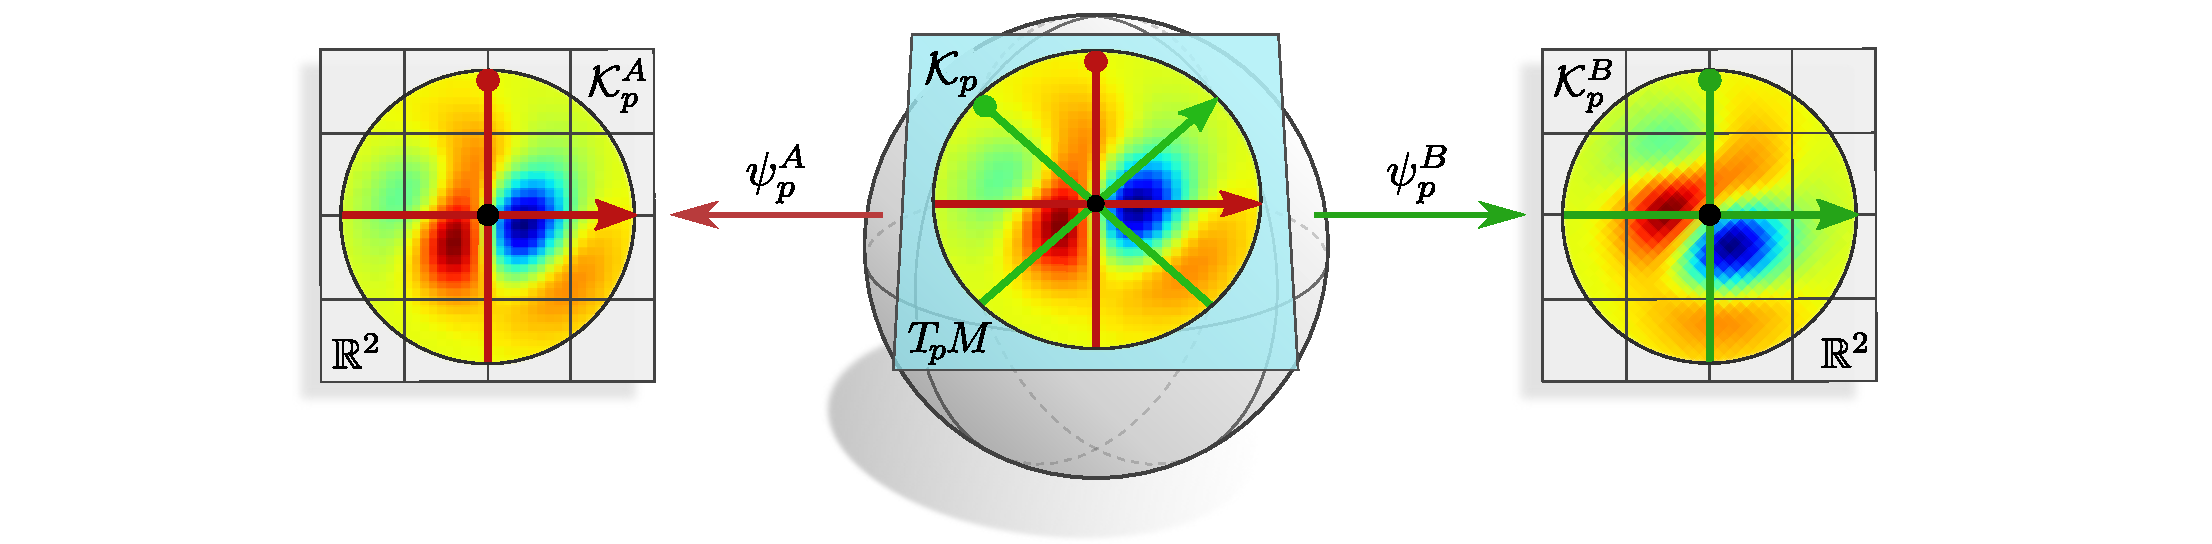
\includegraphics[width=1.\columnwidth]{figures/kernel_apx_coordinatization.pdf}
    \vspace*{-3.5ex}
    \caption{\small
        A \emph{given} coordinate free kernel $\Kp$ on the tangent space $\TpM$ may be represented in arbitrary gauges $\psi_p^A$ or $\psi_p^B$.
        Its coordinate expressions $\Kp^A$ and $\Kp^B$ on $\R^d$ differ in general from each other.
        $G$-steerable kernels have the property to take exactly the same form in all gauges, that is, they satisfy $\Kp^A = \Kp^B = K$ (not visualized).
        }
    \label{fig:kernel_apx_coordinatization}
\end{figure}


\begin{figure}
    \centering
    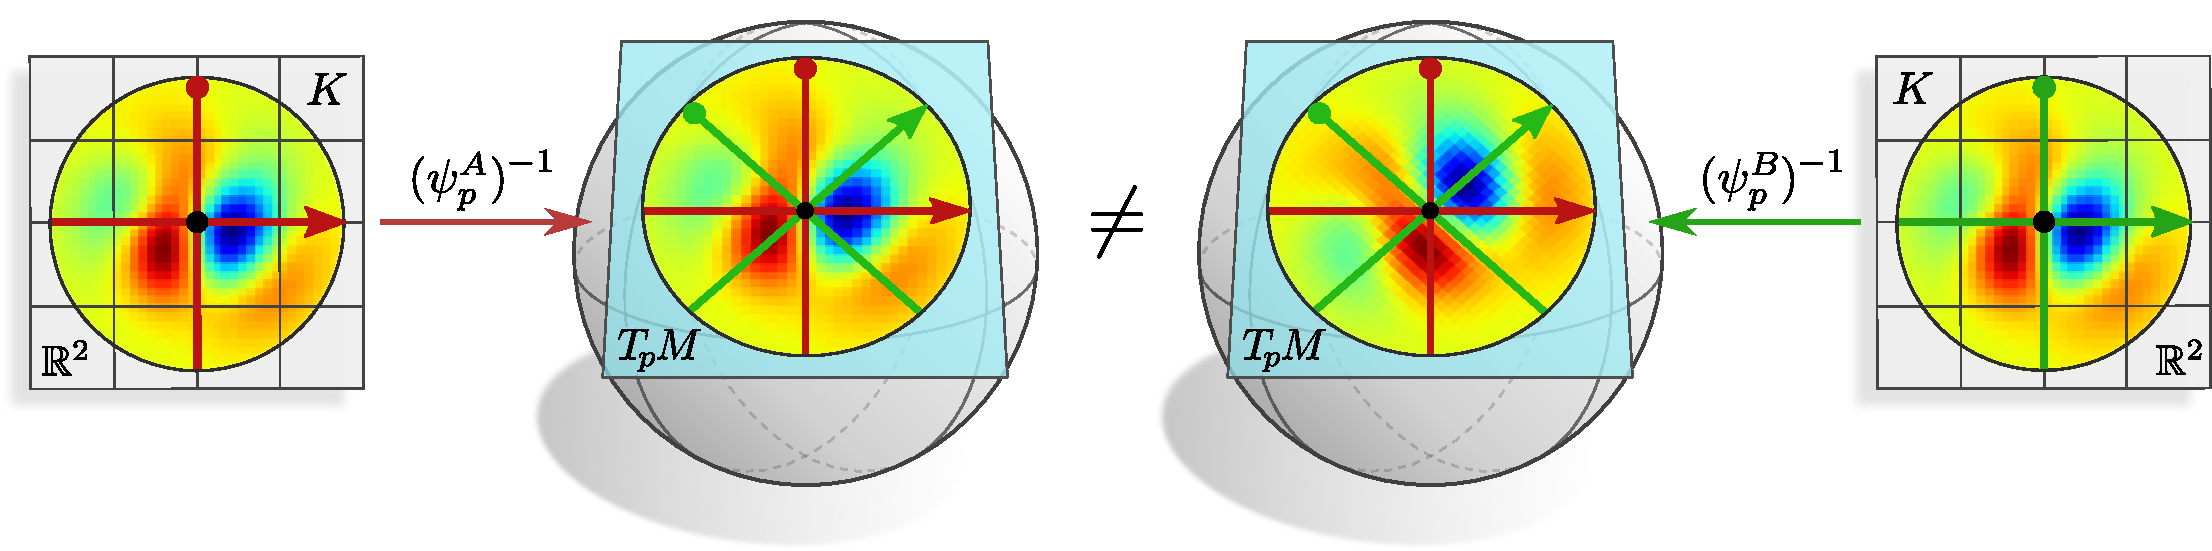
\includegraphics[width=1.\columnwidth]{figures/kernel_apx_sharing.pdf}
    \vspace*{-3.5ex}
    \caption{\small
        A coordinate free kernel may be \emph{defined by sharing} a given kernel $K$ on $\R^d$ relative to some reference frame.
        Different choices of frames result in a different coordinate free kernel.
        $G$-steerable kernels have the property to produce exactly the same coordinate free kernel, independent from the chosen reference frame along which they are shared (not visualized).
        This allows for a coordinate independent weight sharing.
        }
    \label{fig:kernel_apx_sharing}
\end{figure}


A fundamental assumption in the design of $\GM$-convolutions is that kernels $K$ on $\R^d$ are shared relative to some choice of reference frame as visualized in Fig.~\ref{fig:kernel_apx_sharing}.
For general kernels, different choices of frames will lead to different alignments of the resulting coordinate free kernel on the tangent space~$\TpM$
-- the weight sharing process is therefore not coordinate independent.
Fig.~\ref{fig:kernel_apx_coordinatization} shows a different situation:
here we assume a coordinate free kernel $\Kp$ that is already given on~$\TpM$ and express it in different gauges on~$\R^d$.
The coordinate representations $\Kp^A$ and $\Kp^B$ do in general not agree with each other but the construction is coordinate independent.


$G$-steerable kernels are constrained exactly such that they guarantee the coordinate independence of the weight sharing process.
Sharing them relative to different frames results in the same coordinate independent kernel on the tangent space,
that is, there will be no difference between the two kernels in the middle of Fig.~\ref{fig:kernel_apx_sharing}.
Equivalently, the resulting coordinate free kernel on $\TpM$ will take the same form $\Kp^A = \Kp^B = K$ when being expressed in different gauges,
that is, the left and the right kernel in Fig.~\ref{fig:kernel_apx_coordinatization} would agree.


Note that this does not necessarily require the kernel to be invariant in the sense that $K(g\mathscr{v}) = K(\mathscr{v})$ for any $g\in G$ and any~$\mathscr{v}\in\R^d$, as the visual intuition might suggest.
This is indeed a special case for kernels that map between scalar fields, i.e. for which both $\rhoin$ and $\rhoout$ are trivial representations (see e.g. Fig.~\ref{fig:intro_steerable_kernel} for $G=\Flip$ or Fig.~\ref{fig:zonal_kernel} for $G=\O2$).
For more general field types the kernels need to be gauge equivariant, i.e. need to satisfy the $G$-steerability constraint
$K(g\mkern1.5mu \mathscr{v}) = \detg^{-1} \rhoout(g)\: K(\mathscr{v})\: \rhoin(g)^{-1}$
which allows for a steering of the ${\cout\times\cin}$ kernel channels (not visualized).
Of course, $G$-steerable kernels can be interpreted as being gauge \emph{invariant} in the sense that
$K(\mathscr{v}) = \detg \rhoout(g)^{-1}\: K(g\mkern1.5mu \mathscr{v})\: \rhoin(g)$
for any $g\in G$ and any~$\mathscr{v}\in\R^d$.
This notion of gauge invariance allows the coordinate independent sharing of $G$-steerable kernels.


A more detailed discussion of coordinate free kernels and their coordinate expressions is found in Section~\ref{sec:kernel_field_trafos}.
The $G$-steerability constraint is derived in Section~\ref{sec:gauge_conv}.
